\chapter{Memory Management}

The \jr\ has 512 KB of system RAM which can be used for programs, data, and graphics. It also has 512 KB of read-only flash memory that can be used by whatever operating system is installed. Finally, the \jr\ comes with an expansion port and allows for 256KB of expansion RAM to be added. Now, the 65C02 CPU at the heart of the \jr\ has an address space of only 64 KB, so how can it access all this memory, not to mention the I/O devices on the system? The answer is paging. The \jr\ has a special memory management unit (MMU) that can swap banks of memory or I/O registers into and out of the memory space of the CPU.

To understand how it all works, we first need to look at how RAM and flash memory are handled by the \jr. Because there are 1,280 KB of total storage on the system, the system has a 21-bit address bus to manage the memory. RAM and flash have address on that 21-bit bus as shown in table~\ref{tab:memory}.

\begin{table}[ht]
	\begin{center}
		\begin{tabular}{| l | l | l |} \hline
			Start & End & Memory Type \\ \hline\hline
		  	\verb+0x000000+ & \verb+0x07FFFF+ & System RAM (512 KB)\\ \hline
			\verb+0x080000+ & \verb+0x0FFFFF+ & Flash Memory (512 KB) \\ \hline
			\verb+0x100000+ & \verb+0x13FFFF+ & Expansion RAM (256 KB)\\ \hline
		\end{tabular}
	\end{center}
	\caption{\jr\ memory layout}
	\label{tab:memory}
\end{table}

This memory is divided up into ``banks'' of 8 KB each. The 16-bit address space of the CPU is also divided up into 8 KB banks. The MMU allows the program to assign any bank of system memory to any bank of the CPU's memory. It does this through the use of memory look-up tables (LUT), which provide the upper bits needed to select the bank out of system memory for any given bank in CPU memory. It takes 13 bits to specify an address within 8 KB, which means for a 16-bit address from the CPU, the upper 3 bits are the bank number. Since the system bus is 21 bits, the upper 8 bits are used to address the correct 8 KB bank in the full system memory. So a LUT must provide a 8-bit system bank number for each 3-bit bank number provided by the CPU.

NOTE: The original RevA developer's board has a different memory map from the RevB. The RevA does not include an expansion slot and has only 256KB of system RAM. See table~\ref{tab:sys_mem_map_reva} for the overall memory map of the RevA board. Additionally, the RevA bus is only 20-bits wide, and the memory LUTs are only 7 bits wide.

The \jr's MMU supports up to four LUTs, only one of which is active at any given moment. This allows programs to define four different memory layouts and switch between them quickly, without having to alter a LUT on the fly.

\begin{table}[ht]
	\begin{center}
		\begin{tabular}{| c | c || c | c | c | c | c | c | c | c |} \hline
			Bank & A[15..13] & Start & End \\ \hline\hline
			0 & 000 & \verb+0x0000+ & \verb+0x1FFF+ \\ \hline
			1 & 001 & \verb+0x2000+ & \verb+0x3FFF+ \\ \hline
			2 & 010 & \verb+0x4000+ & \verb+0x5FFF+ \\ \hline
			3 & 011 & \verb+0x6000+ & \verb+0x7FFF+ \\ \hline
			4 & 100 & \verb+0x8000+ & \verb+0x9FFF+ \\ \hline
			5 & 101 & \verb+0xA000+ & \verb+0xBFFF+ \\ \hline
			6 & 110 & \verb+0xC000+ & \verb+0xDFFF+ \\ \hline
			7 & 111 & \verb+0xE000+ & \verb+0xFFFF+ \\ \hline
		\end{tabular}
	\end{center}
	\caption{CPU Memory Banks}
	\label{tab:mem_banks}
\end{table}

Of the eight CPU memory banks, one is special. Bank 6 can be mapped to memory as the rest can, or it can be mapped to I/O registers, which are not memory mapped in the same way as RAM and flash. All I/O devices on the \jr\ therefore live within 0xC000 through 0xDFFF on the CPU, but only if the MMU is set to map I/O to bank 6. There is quite a lot of I/O to access on the \jr, so there are four different banks of I/O registers and memory that can be mapped to bank 6 (see table~\ref{tab:io_banks}).

\begin{table}[ht]
	\begin{center}
		\begin{tabular}{| l | l |} \hline
			I/O Bank & Purpose \\ \hline\hline
			0 & Low level I/O registers \\ \hline
			1 & Text display font memory and graphics color LUTs \\ \hline
			2 & Text display character matrix \\ \hline
			3 & Text display color matrix \\ \hline
		\end{tabular}
	\end{center}
	\caption{I/O Banks}
	\label{tab:io_banks}
\end{table}

The MMU is controlled through two main registers, which are always at locations 0x0000 and 0x0001 in the CPU's address space (see table~\ref{tab:mmu_registers}). These registers allow programs to select an active LUT, edit a LUT, and control bank 6:

\begin{table}[ht]
	\begin{center}
		\begin{tabular}{| c | c | c || c | c | c | c | c | c | c | c |} \hline
			Address & R/W & Name & 7 & 6 & 5 & 4 & 3 & 2 & 1 & 0 \\ \hline\hline
			\verb+0x0000+ & RW & MMU\_MEM\_CTRL & EDIT\_EN & --- & \multicolumn{2}{|c|}{EDIT\_LUT} & --- & --- & \multicolumn{2}{|c|}{ACT\_LUT} \\ \hline
			\verb+0x0001+ & RW & MMU\_IO\_CTRL & \multicolumn{5}{|c|}{---} & IO\_DISABLE & \multicolumn{2}{|c|}{IO\_PAGE} \\ \hline
		\end{tabular}
	\end{center}
	\caption{MMU Registers}
	\label{tab:mmu_registers}
\end{table}

\begin{description}
	\item[ACT\_LUT] these two bits specify which LUT (0--3) is used to translate CPU bus address to system bus addresses.

	\item[EDIT\_EN] if set (1), this bit allows a LUT to be edited by the program, and memory addresses 0x0008--0x0010 will be used by the LUT being edited. If clear (0), those memory locations will be standard memory locations and will be mapped like the rest of bank 0.

	\item[EDIT\_LUT] if EDIT\_EN is set, these two bits will specify which LUT (0 - 3) is being edited and will appear in memory addresses 0x0008--0x0010.

	\item[IO\_DISABLE] if set (1), bank 6 is mapped like any other memory bank. If clear (0), bank 6 is mapped to I/O memory.

	\item[IO\_PAGE] if IO\_DISABLE is clear, these two bits specify which bank of I/O memory (0 - 3) is mapped to bank 6.
\end{description}

\example{Setting up a LUT}

In this example, we will set up LUT 1 so that the first six banks of CPU memory map to the first banks of RAM, bank 7 of CPU memory maps to the first bank of flash memory, and bank 6 maps to the first I/O bank.

\begin{verbatim}
    lda #$90      ; Active LUT = 0, Edit LUT#1
    sta $0000

    ldx #0        ; Start at bank 0
l1: txa           ; First 6 banks will just be the first banks of RAM
    sta $0008,x   ; Set the LUT mapping for this bank
    inx           ; Move to the next bank
    cpx #6        ; Until we get to bank 6
    bne l1

    lda #$40      ; Bank 7 maps to $80000, first bank of flash
    sta $000f

    stz $0001     ; Bank 6 should be I/O bank 0

    lda #$01      ; Turn off LUT editing, and switch to LUT#1
    sta $0000
\end{verbatim}

\section*{MMU Boot Configuration}
\label{pg:mmu_boot_config}

While the MMU registers allow the MMU to select one of four memory LUTs to be used for address translation or to be edited, in fact the \jr's MMU actually has eight LUTs in two sets of four. At any given time, only one of those sets of four LUTs is active. One set of LUTs is the ``boot from RAM'' set, and the other is the ``boot from flash'' set. As the names imply, one set is meant to allow you to boot the \jr\ to run code you have loaded into RAM (useful for development and debugging), while the other is meant to be used to boot up an operating system you have loaded into flash memory (useful for just running programs and playing games).

When the \jr\ powers on, it initializes the LUTs in two different ways. The ``boot from RAM'' LUTs are initialized so the 64KB of CPU address space is simply mapped to the first 64KB of system RAM. The ``boot from flash'' LUTs are initialized to be the same, except that the last bank of CPU address space (0xE000 -- 0xFFFF) is mapped to the last bank of flash memory (0x07E000 -- 0x07FFFF). After the LUTs are initialized, the \jr\ checks to see which of the two sets of LUTs should be used and enables them. The memory LUTs that are not selected are completely ignored. See figure ~\ref{fig:lut_choice} to see how the LUTs are related and how they are initialized on power up.

\begin{figure}[ht]
    \begin{center}
        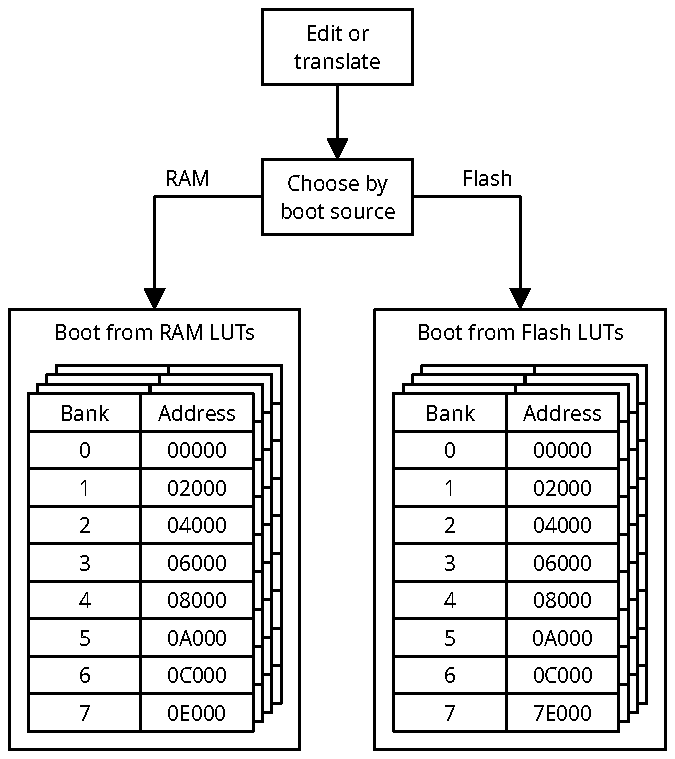
\includegraphics{images/MemoryLUTSelection.pdf}
    \end{center}
    \caption{MMU Boot Configuration}
    \label{fig:lut_choice}
\end{figure}

How the \jr\ decides which set of LUTs to use depends upon the board. The older, RevA boards have a command available over the USB debug port that switches the active LUTs on the fly. The newer, RevB boards have a jumper to choose between the LUTs.

NOTE: the memory LUTs are really just tables stored in RAM in the TinyVicky chip, and apart from the power-up initialization, TinyVicky does not change the LUTs except when directed by a program. Pressing the RESET button does not re-initialize the LUTs. This means that a program should not assume the LUTs are set to any particular value on reset, unless the operating system is initializing the LUTs. A program running as an operating system or even just taking complete control over the board should always initialize the LUTs to the values it needs as one of its first tasks. Of course, a complete power cycle of the board will reset the LUTs, but a program will not always be starting from a complete power cycle.
